\section{Приближение функций. Численные дифференцирование и интегрирование}

\subsection{Интерполяционные многочлены}

\subsubsection{Постановка задачи}
Используя таблицу значений $Y_i$ функции $y = f(x)$, вычисленных в точках $X_i$, $i = 0, \ldots, 3$, построить интерполяционные многочлены Лагранжа и Ньютона, проходящие через точки $\{X_i, Y_i\}$. Вычислить значение погрешности интерполяции в точке $X^*$.

{\bfseries Вариант:}

$y = cos(x)$, $X^* = \frac{\pi}{4}$

\begin{enumerate}
	\item[а).] $X_i = 0, \frac{\pi}{6}, \frac{2\pi}{6}, \frac{3\pi}{6}$
	\item[б).] $X_i = 0, \frac{\pi}{6}, \frac{5\pi}{12}, \frac{\pi}{2}$
\end{enumerate}

\subsubsection{Результаты работы}
\begin{alltt}
$ cat tests/1/1.txt
4
0 0.5235987755982988 1.0471975511965976 1.5707963267948966
0.7853981633974483

$ ./lab3_1 < tests/1/1.txt
Многочлен в форме Лагранжа:
0.1139 * x**3 - 0.6021 * x**2 + 0.0282 * x**1 + 1.0000
Многочлен в форме Ньютона:
0.1139 * x**3 - 0.6021 * x**2 + 0.0282 * x**1 + 1.0000
Погрешность интерполяции:
0.0012
\end{alltt}

\begin{alltt}
$ cat tests/1/2.txt
4
0 0.5235987755982988 1.3089969389957472 1.5707963267948966
0.7853981633974483

$ ./lab3_1 < tests/1/2.txt
Многочлен в форме Лагранжа:
0.1206 * x**3 - 0.6161 * x**2 + 0.0337 * x**1 + 1.0000
Многочлен в форме Ньютона:
0.1206 * x**3 - 0.6161 * x**2 + 0.0337 * x**1 + 1.0000
Погрешность интерполяции:
0.0023
\end{alltt}

\begin{figure}[h]
\centering
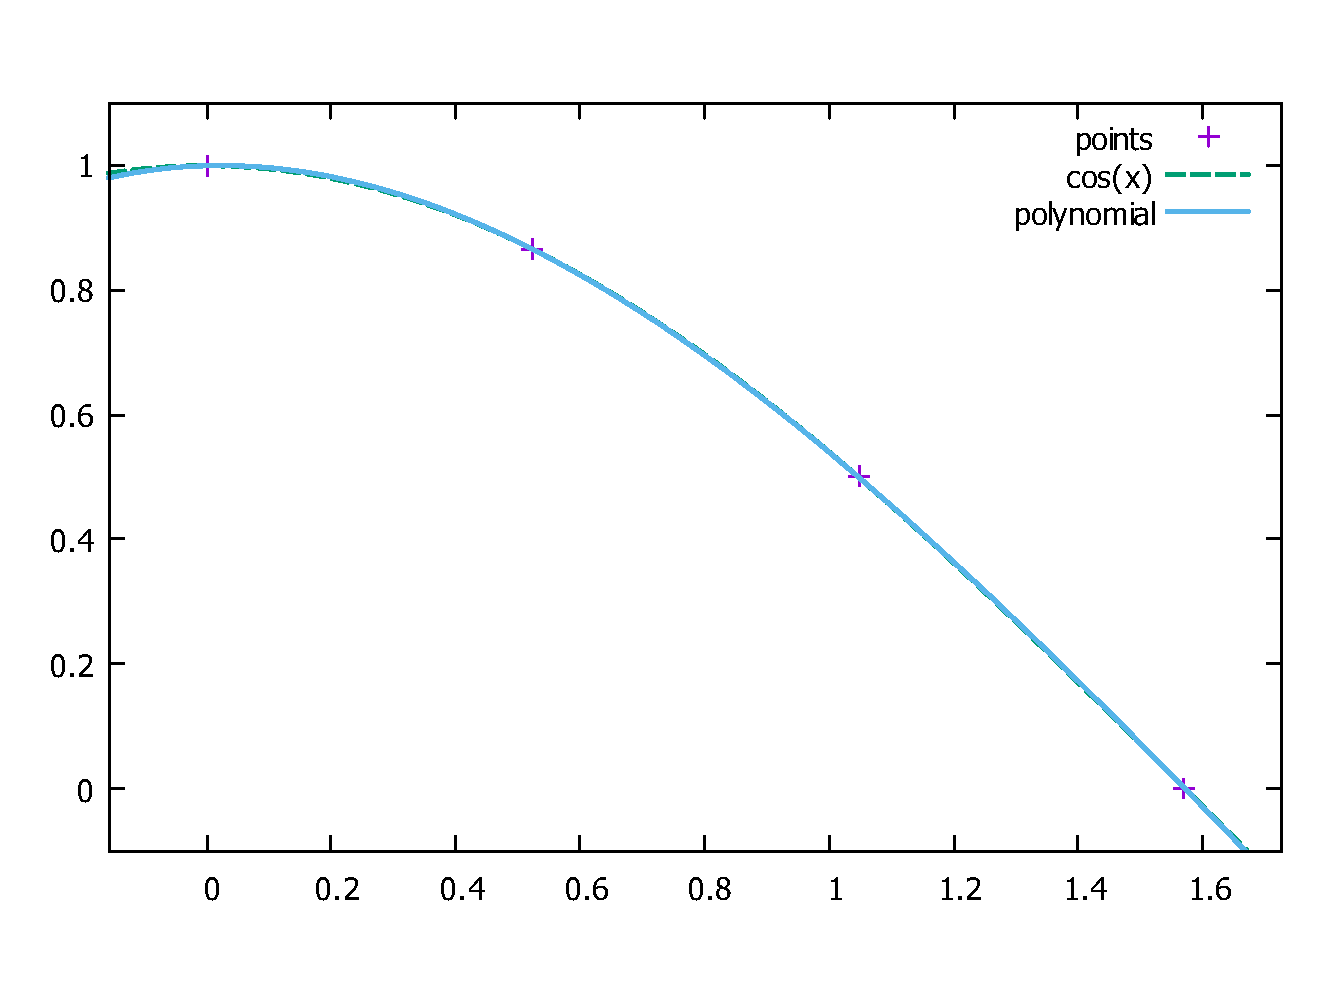
\includegraphics[height=.38\textheight]{lab3_1_1}
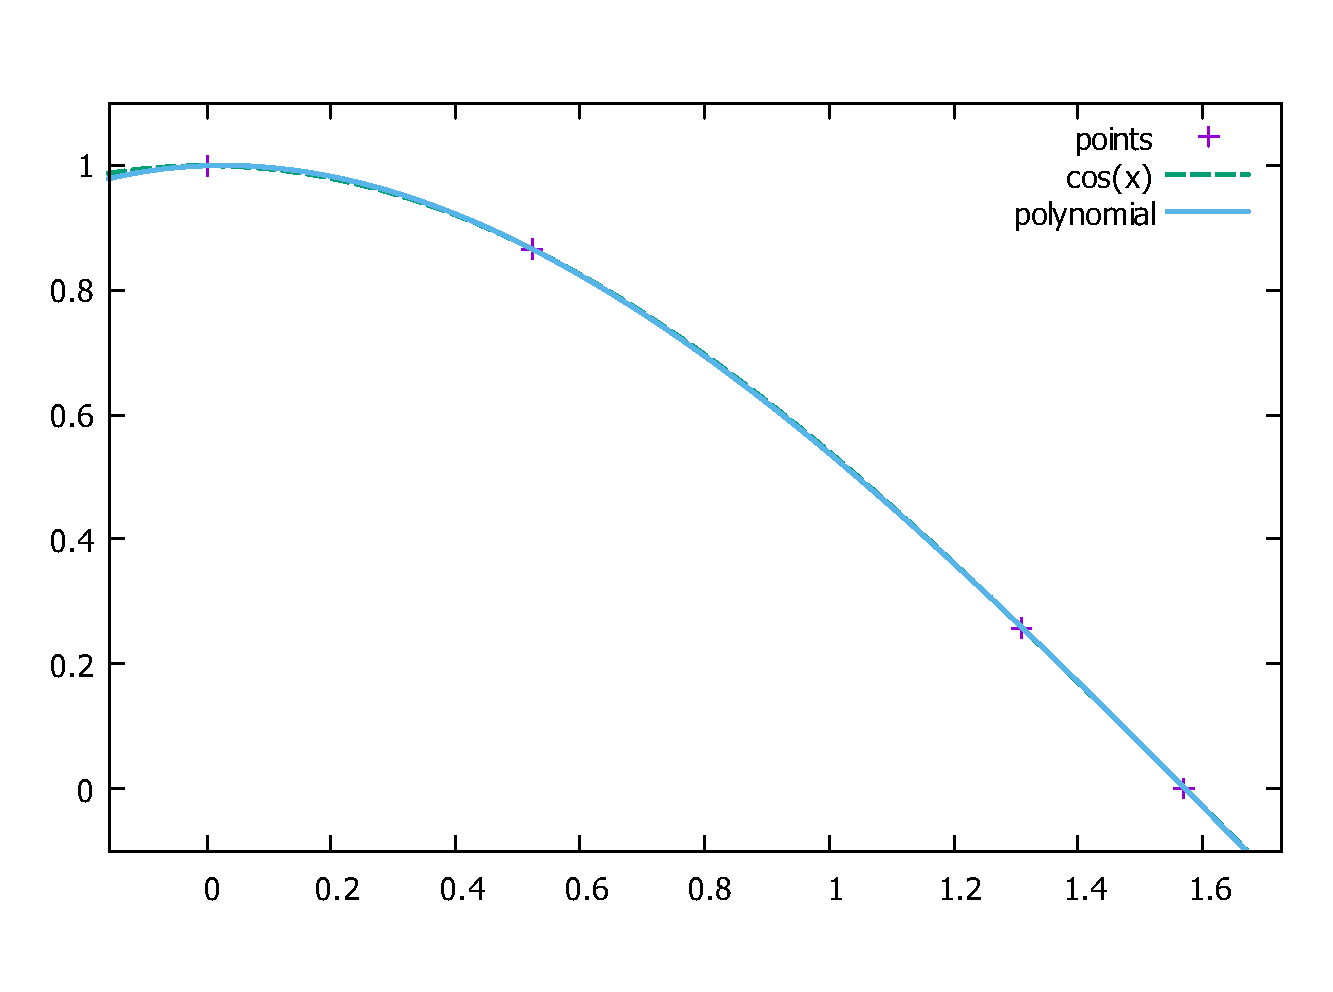
\includegraphics[height=.38\textheight]{lab3_1_2}
\end{figure}
\pagebreak

\subsubsection{Исходный код}
\lstinputlisting{../include/function/interpolation_polynomial.hpp}
\pagebreak

\subsection{Интерполяция кубическими сплайнами}

\subsubsection{Постановка задачи}
Построить кубический сплайн для функции, заданной в узлах интерполяции, предполагая, что сплайн имеет нулевую кривизну при $x = x_0$ и $x = x_4$. Вычислить значение функции в точке $x = X^*$

{\bfseries Вариант:} $X^* = 1.5$

\begin{tabular}{ |c|c|c|c|c|c| }
\hline
$i$ & 0 & 1 & 2 & 3 & 4 \\
\hline
$x_i$ & 0.0 & 1.0 & 2.0 & 3.0 & 4.0 \\
\hline
$f_i$ & 1.0 & 0.86603 & 0.5 & 0.0 & -0.5 \\
\hline
\end{tabular}

\subsubsection{Результаты работы}
\begin{alltt}
$ ./lab3_2 < tests/2/2.txt
Значение в точке 1.5000: 0.7109
Сегменты кубического сплайна:
[0.0000:1.0000] - 0.0526 * x**3 + 0.0000 * x**2 - 0.0814 * x**1 + 1.0000
[1.0000:2.0000] 0.0309 * x**3 - 0.2504 * x**2 + 0.1691 * x**1 + 0.9165
[2.0000:3.0000] 0.0271 * x**3 - 0.2279 * x**2 + 0.1239 * x**1 + 0.9466
[3.0000:4.0000] - 0.0054 * x**3 + 0.0651 * x**2 - 0.7550 * x**1 + 1.8255
\end{alltt}

\begin{center}
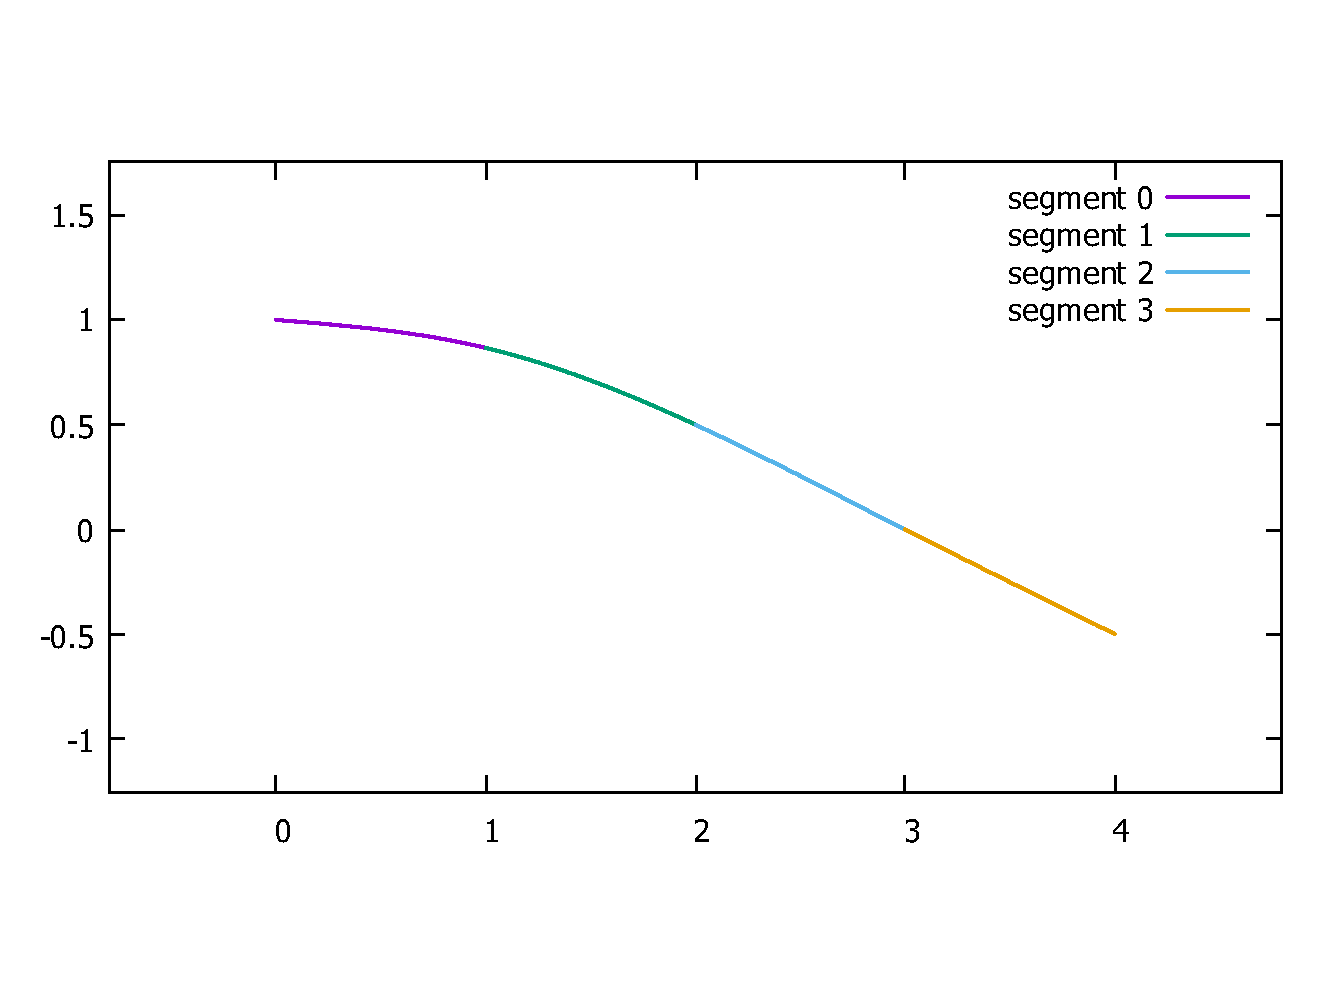
\includegraphics[scale=0.6]{lab3_2}
\end{center}
\pagebreak

\subsubsection{Исходный код}
\lstinputlisting{../include/function/spline.hpp}
\pagebreak

\subsection{Метод наименьших квадратов}

\subsubsection{Постановка задачи}
Для таблично заданной функции путем решения нормальной системы МНК найти приближающие многочлены a) 1-ой и б) 2-ой степени. Для каждого из приближающих многочленов вычислить сумму квадратов ошибок. Построить графики приближаемой функции и приближающих многочленов.

{\bfseries Вариант:}

\begin{tabular}{ |c|c|c|c|c|c|c| }
\hline
$i$ & 0 & 1 & 2 & 3 & 4 & 5\\
\hline
$x_i$ & -1.0 & 0.0 & 1.0 & 2.0 & 3.0 & 4.0 \\
\hline
$f_i$ & 0.86603 & 1.0 & 0.86603 & 0.50 & 0.0 & -0.5 \\
\hline
\end{tabular}

\subsubsection{Результаты работы}
\begin{alltt}
$ ./lab3_3 < tests/3/2.txt
Приближающий многочлен 1-ой степени:
- 0.2913 * x**1 + 0.8923
Ошибка: 0.2708
Приближающий многочлен 2-ой степени:
- 0.0827 * x**2 - 0.0431 * x**1 + 0.9475
Ошибка: 0.0152
Приближающий многочлен 3-ой степени:
0.0151 * x**3 - 0.1508 * x**2 - 0.0174 * x**1 + 1.0110
Ошибка: 0.0003
\end{alltt}
\pagebreak

\begin{center}
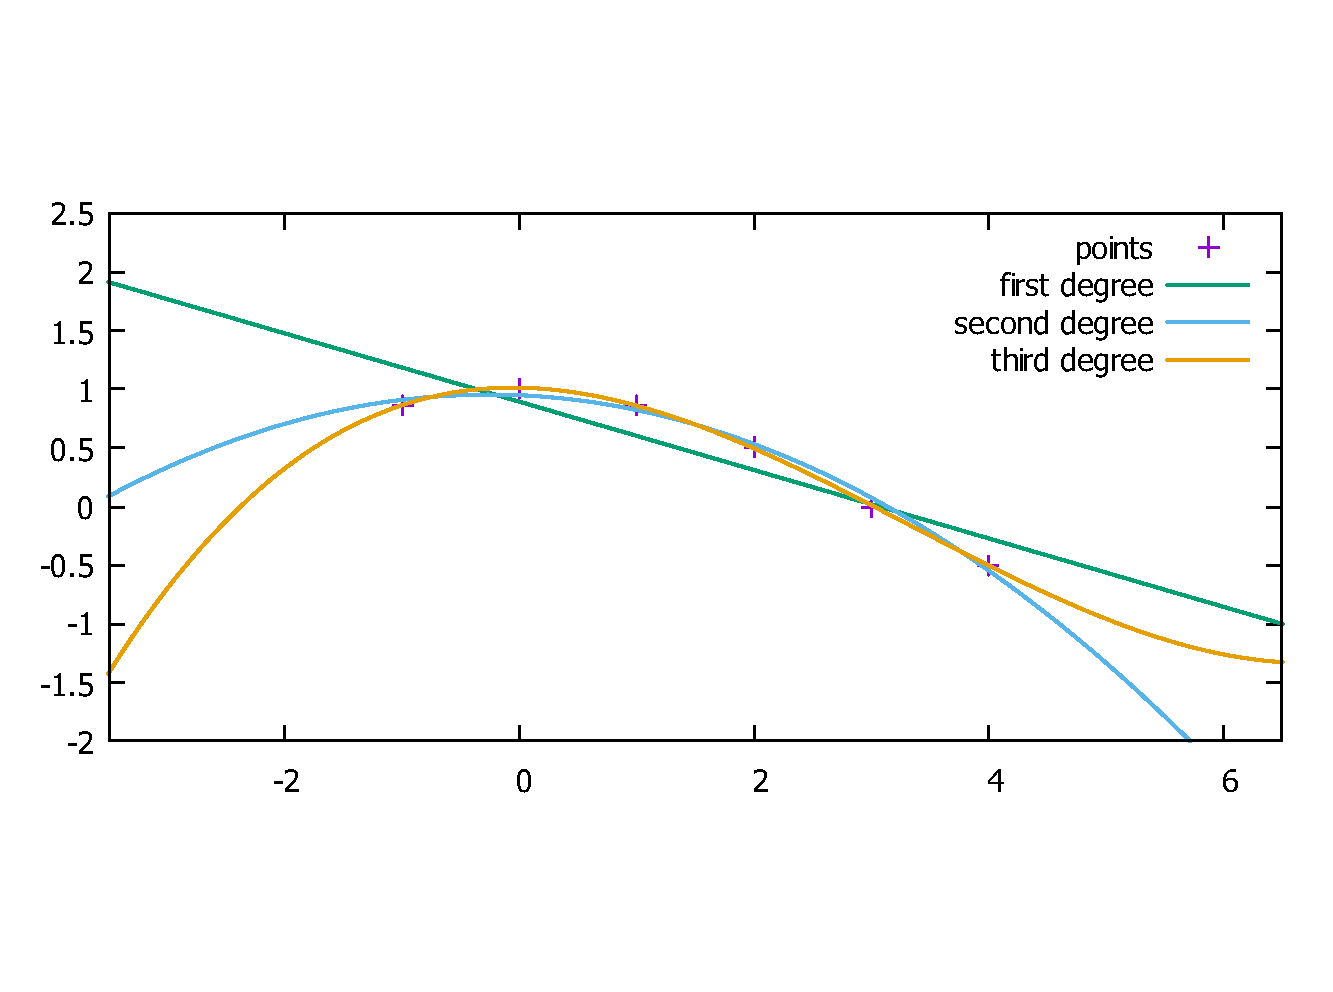
\includegraphics[width=.8\textwidth]{lab3_3}
\end{center}

\subsubsection{Исходный код}
\lstinputlisting{../include/function/lsm.hpp}
\pagebreak

\subsection{Численное дифференцирование}

\subsubsection{Постановка задачи}
Вычислить первую и вторую производную от таблично заданной функции $y_i = f(x_i)$, $i = 0, \ldots, 4$ в точке $x = X^*$.

{\bfseries Вариант:} $X^* = 1.0$

\begin{tabular}{ |c|c|c|c|c|c| }
\hline
$i$ & 0 & 1 & 2 & 3 & 4 \\
\hline
$x_i$ & -1.0 & 0.0 & 1.0 & 2.0 & 3.0 \\
\hline
$f_i$ & -0.5 & 0.0 & 0.5  & 0.86603 & 1.0 \\
\hline
\end{tabular}

\subsubsection{Результаты работы}
\begin{alltt}
$ ./lab3_4 < tests/4/2.txt
Первая производная: 0.4330
Вторая производная: -0.1340
\end{alltt}

\begin{center}
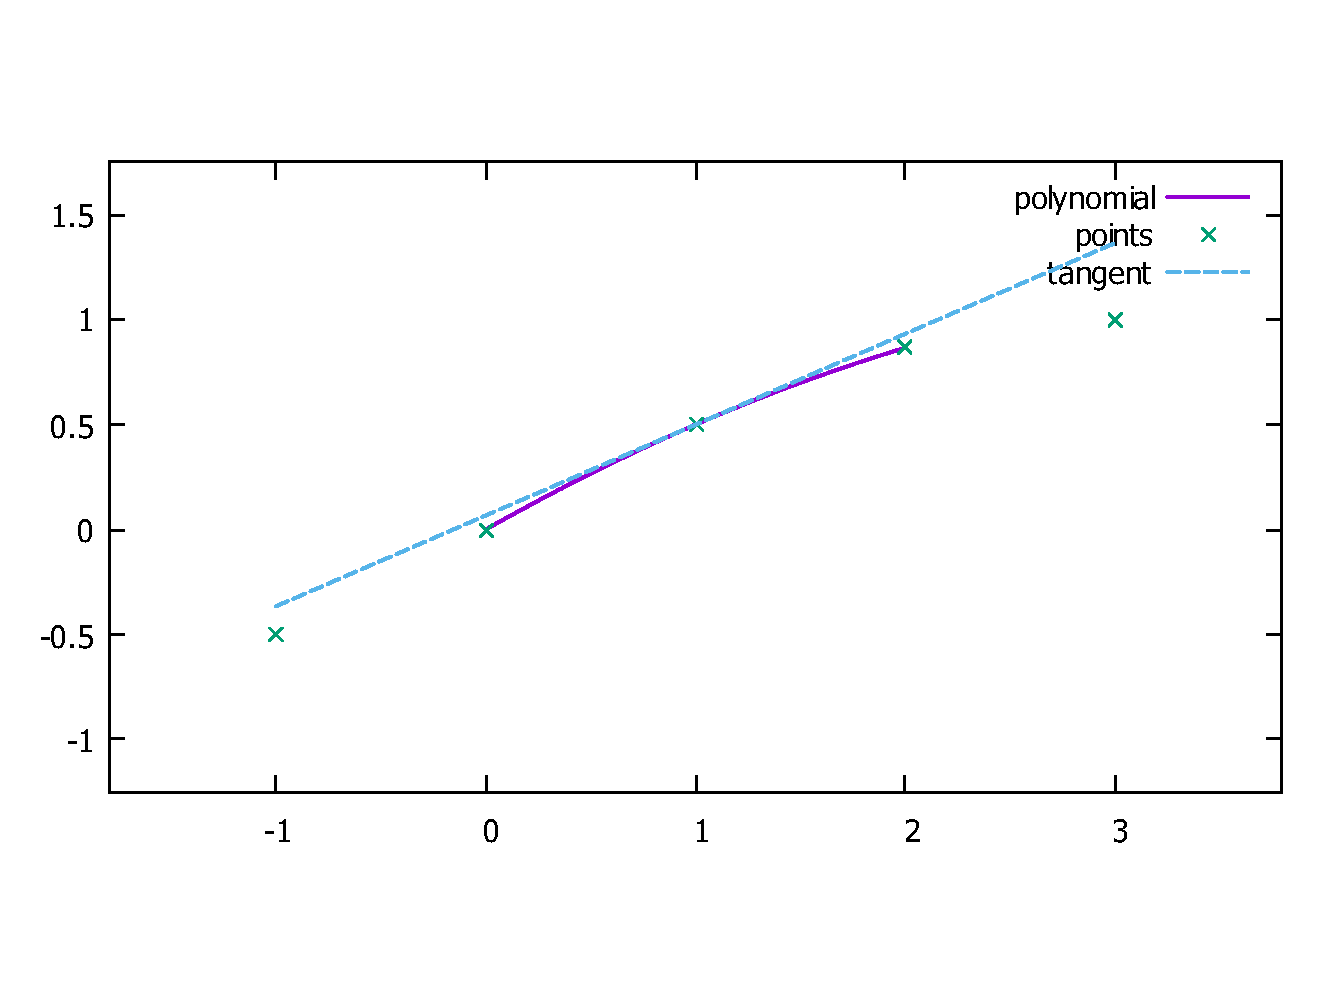
\includegraphics[scale=0.7]{lab3_4}
\end{center}
\pagebreak

\pagebreak

\subsubsection{Исходный код}
\lstinputlisting{../include/function/derivation.hpp}
\pagebreak

\subsection{Численное интегрирование}

\subsubsection{Постановка задачи}
Вычислить определенный интеграл $\int_{X_0}^{X_1}{y dx}$, методами прямоугольников, трапеций, Симпсона с шагами $h_1$, $h_2$. Оценить погрешность вычислений, используя Метод Рунге-Ромберга:

{\bfseries Вариант:}
$$y = \frac{x}{(3x+4)^2},\ X_0 = 0,\ X_1 = 4,\ h_1 = 1.0,\ h_2 = 0.5$$

\subsubsection{Результаты работы}
\begin{alltt}
$ cat tests/5/1.txt
0 4 1

$ ./lab3_5 < tests/5/1.txt
Метод прямоугольников: 0.05816
Погрешность: 0.01816

Метод трапеций: 0.06597
Погрешность: 0.00345

Метод Симпсона: 0.06942
Погрешность: 0.00038

$ cat tests/5/2.txt
0 4 0.5

$ ./lab3_5 < tests/5/2.txt
Метод прямоугольников: 0.06550
Погрешность: 0.00734

Метод трапеций: 0.06941
Погрешность: 0.00114

Метод Симпсона: 0.07055
Погрешность: 0.00008

\end{alltt}
\pagebreak

\subsubsection{Исходный код}
\lstinputlisting{../include/function/integration.hpp}
\pagebreak